\Subsection{Несобственные интегралы}
%BEGIN TICKET 20
\begin{definition}
    Пусть $-\infty < a < b \le +\infty$ и $f \in C[a, b)$.

    Тогда определим  $\int\limits_a^{\to b} f\coloneqq \lim\limits_{B \to b-} \int\limits_a^B f$.

    Если $-\infty \le a < b < +\infty, f \in C(a, b]$, тогда $\int\limits_{\to a}^b f \coloneqq \lim\limits_{A \to a+} \int\limits_A^b f$.
\end{definition}
\begin{remark}
    Если $b < +\infty$ и  $f \in C[a, b]$, то определение не дает ничего нового:  \begin{align*}
        \int_a^b f &= \lim_{B \to b}f \\
        \left|\int_a^b f - \int_a^B f\right| &= \left| \int_B^b f \right| \le M(b-B) \to 0, M = \max\limits_{x \in [a, b]} f(x)
    .\end{align*}
\end{remark}
\begin{example}
    \begin{enumerate}
        \item $\int\limits_1^{+\infty} \frac{\mathrm{d}x}{x^p} = \lim\limits_{y \to +\infty} \int\limits_a^y \frac{\mathrm{d}x}{x^p} = \lim\limits_{\substack{y \to +\infty \\ \text{при}\ p \neq 1}} -\frac{1}{(p-1)x^{p-1}}\mid_{x=1}^{x=y} = \frac{1}{p-1} - \lim\limits_{y \to +\infty} \frac{1}{(p-1)y^{p-1}} = \frac{1}{p-1}$ при $p > 1$, при $p < 1$ получаем $+\infty$, а при $p = 1$  $\lim\limits_{y \to +\infty} \ln x \mid_1^y = \lim\limits_{y \to +\infty} \ln y = +\infty$
        \item $\int\limits_0^1 \frac{\mathrm{d}x}{x^p} = \lim\limits_{y \to 0+} \int\limits_y^1 \frac{\mathrm{d}x}{x^p} = \lim \limits_{y \to 0+} -\frac{1}{(p-1)x^{p-1}} \mid_{x=y}^{x=1} = -\frac{1}{p - 1} + \lim\limits_{y \to 0+} = \frac{y^{1-p}}{p - 1} = \frac{1}{1 - p}$ при $p < 1$, при  $p > 1$ получаем  $+\infty$, а вот при  $p = 1$  $\lim\limits_{y \to 0+} \ln x \mid_y^1 = \lim\limits_{y \to 0+} - \ln y = +\infty$.

            То есть, при  $p < 1$  $\int\limits_0^1 \frac{\mathrm{d}x}{x^p} = \frac{1}{1 - p}$, \\
            при $p \ge 1$ $\int\limits_0^1 \frac{\mathrm{d}x}{x^p} = +\infty$.
    \end{enumerate}
\end{example}
\begin{remark}
    Если $f \in C[a, b)$ и  $F$ его первообразная, то  $\int\limits_a^b f = \lim\limits_{B \to b-}F(B) - F(a)$.

    Если $f \in C[a, b)$ и  $F$ его первообразная, то  $\int\limits_a^b f = F(b) - \lim\limits_{A \to a+}F(A)$.
\end{remark}
\begin{proof}
    Очевидно по формуле Ньютона-Лейбница.
\end{proof}
\begin{definition}
    $F \Big|_a^b \coloneqq \lim\limits_{B \to b-} F(B) - F(a)$.
\end{definition}

\begin{definition}
    $\int\limits_a^{\to b} f$ сходится, если  $\lim B$ в его определении существует и конечен.
\end{definition}

\begin{theorem}[Критерий Коши]
    Пусть $-\infty < a < b \le +\infty$, $f \in C[a, b)$.

    Тогда $\int\limits_a^b f$ сходится  $\iff \forall \eps \exists c \in (a, b)\!: \forall A, B \in (c, b)\ \left|\int\limits_A^B f\right| < \eps$. 
\end{theorem}
\begin{remark}
    \begin{enumerate}
        \item Если $b = +\infty$ это означает, что  $\forall \eps \exists c > a \forall A, B > c\!: \left| \int\limits_A^B f \right|  < \eps$.
        \item  Если $b < +\infty$ это означает, что  $\forall \eps > 0 \exists \delta > 0 \forall A, B \in (b-\delta; b)\!: \left|\int\limits_A^B f \right| < \eps$.
    \end{enumerate}
\end{remark}
\begin{proof}
    Для $b < +\infty$. 
      \begin{itemize}
          \item "$\Rightarrow$" $\int\limits_a^b f$ сходится  $\implies \exists$ конечный  $I \coloneqq \lim\limits_{B \to b-} \int\limits_a^B f$, обозначим $\int\limits_a^B f$ за  $g(B)$. Воспользуемся критерием Коши для функций:

              \[\forall \eps > 0 \exists \delta > 0 \begin{array}{lc} 
              \forall B \in (b - \delta, b) & |g(B) - I| < \frac{\eps}{2}\\ 
          \forall A \in(b - \delta, b) & |g(A) - I| < \frac{\eps}{2}\end{array} \implies |g(B) - g(A)| \le |g(B) - I| + |I - g(A)| < \eps\]
      \item "$\Leftarrow$" $\int\limits_a^B f \eqqcolon g(B)$.

          $\forall \eps > 0 \exists \delta > 0 \forall A, B \in (b-\delta, b)\!: |g(B)- g(A)| < \eps$ это условие из критерия Коши для $\lim\limits_{B \to b-} g(B)$.
  \end{itemize}
\end{proof}
\begin{remark}
    Если существует $A_n, B_n \in [a, b)\!: \lim A_n = \lim B_n = b\!: \int\limits_{A_n}^{B_n} f \centernot\to 0$, то  $\int\limits_a^b f$ расходится.
\end{remark}
\begin{proof}
    Возьмем $A_{n_k}$ и  $B_{n_k}\!: |\int\limits_{A_{n_k}}^{B_{n_k}} f| \to C > 0 \implies |\int\limits_{A_{n_k}}^{B_{n_k}} f| > \frac{C}{2}$ при больших $k$. Но это противоречит критерию Коши.
\end{proof}
%END TICKET 20
%BEGIN TICKET 21
\begin{properties}[несобственных интегралов]
    \begin{enumerate}
        \item Аддитивность. Пусть $f \in C[a, b)$,  $c \in (a, b)$. Если  $\int\limits_a^b f$ сходится, то  $\int\limits_c^b f$ сходится и  $\int\limits_a^b f = \int\limits_a^c f + \int\limits_c^b f$.
        \item Если $\int\limits_a^b f$ сходится, то  $\lim\limits_{c \to b-} \int\limits_c^b f = 0$
        \item Линейность $\alpha, \beta \in \R$ и $\int\limits_a^b f$ и  $\int\limits_a^b g$ сходятся. Тогда  $\int\limits_a^b(\alpha f + \beta g)$ сходится и $\int\limits_a^b (\alpha f + \beta g) = \alpha \int\limits_a^b f + \beta\int\limits_a^b g$.
        \item Монотонность. Пусть $\int\limits_a^b f$ и $\int\limits_a^b g$ существует в  $\overline{R}$ и  $f \le g$ на $[a, b)$. Тогда  $\int\limits_a^b f \le \int\limits_a^b g$.
        \item Интегрирование по частям. $f, g \in C^1[a; b) \implies \int\limits_a^b fg' = fg \Big|_a^b - \int\limits_a^b f'g$.
        \item Замена переменных. $\vphi\!: [\alpha, \beta) \to [a, b)$,  $\vphi \in C^1[\alpha, \beta)$ и $\exists \lim\limits_{\gamma \to \beta-} \vphi(\gamma) \eqqcolon \vphi(\beta-)$ и $f \in C[a, b)$.

            Тогда  $\int\limits_\alpha^\beta f(\vphi(t)) \vphi'(t)\mathrm{d}t = \int\limits_{\vphi(\alpha)}^{\vphi(\beta-)} f(x) \mathrm{d}x$. <<Если существует один из  $\int$, то существует второй и они равны>>
    \end{enumerate}
\end{properties}
\begin{proof}
    \begin{enumerate}
        \item $\int\limits_a^b f = \lim\limits_{B \to b-} F(B) - F(a) \implies \lim_{B \to b-}F(B)$ существует и конечный  $\implies \int\limits_c^b = \lim\limits_{B \to b-} F(b) - F(c)$ --- сходится.

            $\int\limits_a^b = \lim F(B) - F(a) = \lim F(B) - F(c) + F(c) - F(a) = \int\limits_c^b f + \int\limits_a^c f$.
        \item $\int\limits_c^b f = \int\limits_a^b f- \int\limits_a^c f \to \int\limits_a^b f - \int\limits_a^b f = 0$
        \item $\int\limits_a^b (\alpha f + \beta g) = \lim\limits_{B \to b-} \int\limits_a^B(\alpha f + \beta g) = \lim\limits_{B \to b-}(\alpha \int\limits_a^B f + \beta \int\limits_a^B g) = \alpha \lim\limits_{B \to b-} \int\limits_a^B f + \beta\lim\limits_{B \to b-} \int\limits_a^B g = \alpha \int\limits_a^b f + \beta \int\limits_a^b g$.
        \item $\int\limits_a^B f \le \int\limits_a^B g$ (монотонность интеграла), а дальше предельный переход.
        \item $a < B < b$. $\int\limits_a^B fg' = fg \Big|_a^B - \int\limits_a^B f'g$ и переход к пределу. Так как $f, g$ --- непрерывные функции, то  $\lim\limits_{B \to b-} fg\Big|_a^B = fg \Big|_a^b$, а интеграл по определению.
        \item $F(y) \coloneqq \int\limits_{\vphi(\alpha)}^y f(x) \mathrm{d}x$,  $\Phi(\gamma) \coloneqq \int_{\alpha}^{\gamma} f(\vphi(t)) \vphi'(t) \mathrm{d}t$. Знаем, что $F(\vphi(\gamma)) = \Phi(\gamma)$ при  $\alpha < \gamma < \beta$.

            Пусть существует правый  $\int$, то есть  $\exists \lim\limits_{y \to \vphi(\beta-)} F(y)$. Возьмем  $\gamma_n \nearrow \beta \implies \vphi(\gamma_n) \to \vphi(\beta-) \implies \Phi(\gamma_n) = F(\vphi(\gamma_n)) \to \int\limits_{\vphi(\alpha)}^{\vphi(\beta-)} f(x) \mathrm{d}x$. При этом $\Phi(\gamma_n) \to \int\limits_{\alpha}^{\beta} f(\vphi(t))\vphi'(t)\mathrm{d}t$.

            Пусть существует левый $\int$, то есть  $\exists \lim\limits_{\gamma \to \beta-} \Phi(\gamma)$. Докажем, что  $\exists$ правый  $\int$. При  $\vphi(\beta-) < b$ нечего доказывать. 

            Пусть  $\vphi(\beta-) = b$. Тогда  возьмем $b_n \nearrow b$. Можно считать, что $b_n \in [\vphi(\alpha), b)$. Тогда $\exists \gamma_n \in [\alpha, \beta)\!: \vphi(\gamma_n) = b_n$. Докажем, что  $\gamma_n \to \beta$. Пусть это не так. Тогда найдется  $\gamma_{n_k} \to \widetilde{\beta} < \beta \implies \vphi(\gamma_{n_k}) \to \vphi(\widetilde{\beta}) < b$ по непрерывности в  $\widetilde{\beta}$. Противоречие.

            Итак,  $\gamma_n \to \beta$,  $F(b_n) = F(\vphi(\gamma_n)) = \Phi(\gamma_n) \to \int\limits_\alpha^\beta f(\vphi(t))\vphi'(t) \mathrm{d}t$.
    \end{enumerate}
\end{proof}
\begin{remark}[ко второму свойству]
    \begin{enumerate}
        \item Если  $\int\limits_a^b f$ сходится, а  $\int\limits_a^b g$ расхоидится, то  $\int\limits_a^b (f+g)$ расходится. Доказательство от противного, путь интеграл сходится, то  $g = (f+g)-f \implies \int\limits_a^b g$ сходится.
        \item Если $\int\limits_a^b f$ и  $\int\limits_a^b g$ расходятся, то  $\int\limits_a^b (f+g)$ может сходиться.  $\int\limits_1^{+\infty} \frac{\mathrm{d}x}{x}$ и $\int\limits_1^{+\infty} -\frac{\mathrm{d}x}{x}$ расходятся.
    \end{enumerate}
\end{remark}
\begin{remark}[к шестому свойству]
    $\int\limits_a^b f(x) \mathrm{d}x$. Сделаем замену  $x = b - \frac{1}{t} = \vphi(t)$, $\vphi'(t) = \frac{1}{t^2}, \vphi(\alpha) = a, \alpha = \frac{1}{b-a}$.

    Тогда $\int\limits_a^b f(x) \mathrm{d}x = \int\limits_{\frac{1}{b-a}}^{+\infty} f(b-\frac{1}{t}) \frac{1}{t^2} \mathrm{d}t$.
\end{remark}

\begin{definition}
    Пусть $f$ непрерывен на  $(a, b)$ за исключением точек  $c_1 < c_2 < \ldots < c_n$.

    $\int\limits_a^b f$ сходится, если сходятся интегралы по все маленьким отрезкам (содержащих только одну выколотую точку).
\end{definition}
%END TICKET 21
\subsection*{Несобственные интегралы от неотрицательных функций}
%BEGIN TICKET 22
\begin{theorem}
    Пусть  $f \in C[a, b)$ и  $f \ge 0$. 

    Тогда $\int\limits_a^b f$ сходится  $\iff F(y) \coloneqq \int\limits_a^y f$ ограничена сверху.
\end{theorem}
\begin{proof}
    $f \ge 0 \implies F$ монотонно возрастает. $\int\limits_a^b f$ сходится  $\iff \exists$ конечный  $\lim\limits_{y \to b-}F(y) \iff F$ ограничена сверху. 
\end{proof}
\begin{remark}
    $f \in C[a; b), f\ge 0$. $\int\limits_a^b f$ расходящийся означает, что  $\int\limits_a^b f = +\infty$.
\end{remark}
\begin{consequence}[Признак сравнения]
    $f, h \in C[a, b)$,  $f, g \ge 0$ и $f \le g$.
    \begin{enumerate}
        \item Если $\int\limits_a^b g$ сходится, то  $\int\limits_a^b f$ сходится.
        \item Если  $\int\limits_a^b f$ расходится, то  $\int\limits_a^b g$ расходится.
    \end{enumerate}
\end{consequence}
\begin{proof}
    $F(y) \coloneqq \int\limits_a^y f$ и  $G(y) \coloneqq \int\limits_a^y g$.
     \begin{enumerate}
         \item Пусть $\int\limits_a^b g$ сходящийся  $\implies$  $G(y)$ ограничена, но  $F(y) \le G(y) \implies F(y)$ ограничена $\implies \int\limits_a^b f$ сходящаяся.
         \item От противного.
    \end{enumerate}
\end{proof}
\begin{remark}
    \begin{enumerate}
        \item Неравенство $f \le g$ нужно лишь для аргументов близких к $b$.
        \item Неравенство  $f \le g$ можно заменить на $f = \mathcal{O}(g)$.

            $f = \mathcal{O}(g) \implies f \le cg$. $\int\limits_a^b g$ сходящийся  $\implies \int\limits_a^b cg $ сходящийся  $\implies \int\limits_a^b f$ -- сходящийся.
        \item Если  $f = \mathcal{O}(\frac{1}{x^{1 + \eps}})$ для $\eps > 0$, то  $\int\limits_a^{+\infty} f$ --- сходящийся.

            $g(x) = \frac{1}{x^{1+\eps}}$ и можно считать, что $a \ge 1$ $\int\limits_a^{+\infty} g(x) \mathrm{d}x$ --- сходящийся.
    \end{enumerate}
\end{remark}
\begin{consequence}
    $f, g \in C[a, b)$,  $f, g \ge 0$ и $f(x) \sim g(x), x \to b-$. Тогда  $\int\limits_a^b f$ и  $\int\limits_a^b g$ ведут себя одинаково (либо оба сходятся, либо оба расходятся).
\end{consequence}
\begin{proof}
    $f \sim g \implies f = \vphi \cdot g$, где  $\vphi(x) \xrightarrow{x \to b-} 1 \implies$ в окрестности $b$  $\frac{1}{2} \le \vphi \le 2 \implies f \le 2g \land g \le 2f$ в окрестности $b$  $\implies$ из сходимости интеграла  $g$ следует сходимость $f \land$ наоборот. 
\end{proof}
%END TICKET 22
%BEGIN TICKET 23
\begin{definition}
    $f \in C[a, b)$. $\int\limits_a^b f$ абсолютно сходится, если  $\int\limits_a^b |f|$ сходится.
\end{definition}
\begin{theorem}
    $\int\limits_a^b f$ сходится абсолютно  $\implies \int\limits_a^b f$ сходится.
\end{theorem}
\begin{proof}
    $f = f_+ - f_-$,  $|f| = f_+ + f_-$.  $|f| \ge f_\pm \ge 0$. Если $\int\limits_a^b f$ сходится абсолютно  $\implies \int\limits_a^b$ сходится  $\int\limits_a^b f_{\pm}$ сходится  $\implies \int\limits_a^b f = \int\limits_a^b f_+ - \int\limits_a^b f_-$ сходящийся.
\end{proof}
\begin{theorem}[Признак Дирихле]
    $f, g \in C[a, +\infty)$. Если
    \begin{enumerate}
        \item $f$ имеет ограниченную на  $[a, +\infty]$ первообразную, то есть  $\left| \int\limits_a^y f(x) \mathrm{d}x \right| \le K \quad \forall y$.
        \item $g$ монотонна.
        \item  $\lim\limits_{x \to +\infty} g(x) = 0$
    \end{enumerate}, то $\int\limits_a^{+\infty} f(x)g(x) \mathrm{d}x$ сходится.
\end{theorem}
\begin{proof}
    Только для случая $g \in C^1[a; +\infty)$. 

    Надо доказать, что  $\exists$ конечный  $\lim\limits_{y \to +\infty} \int\limits_a^y f(x)g(x) \mathrm{d}x$,  $F(y) \coloneqq \int\limits_a^y f(x)\mathrm{d}x$. 
    \begin{align*}
        \int\limits_a^y f(x)g(x)\mathrm{d}x = \int\limits_a^y F'(x)g(x) \mathrm{d}x = F(x)g(x) \Big|_a^y - \int_a^y F(x) g'(x) \mathrm{d}x = F(y)g(y) - \int_a^y F(x)g'(x) \mathrm{d}x
    \end{align*}

    Чтобы доказать существование предела у разности каких-то штук, нужно доказать, что он существует у них по отдельности.

    $\lim\limits_{y \to +\infty} F(y)g(y) = 0$ --- произведение бесконечно малой и ограниченной функции.

    Хотим показать, что $\int\limits_a^y F(x)g'(x)\mathrm{d}x$ имеет конечный  $\lim$, то есть  $\int\limits_a^{+\infty} F(x)g'(x) \mathrm{d}x$ сходится.

    Тогда докажем, что он абсолютно сходится.  $\int\limits_a^{+\infty} |F(x)| |g'(x)| \mathrm{d}x$, $|F(x)||g'(x)| \le K|g'(x)| = Kg'(x)$. (считаем, что $g(x)$ возрастает) $\int_a^{+\infty} g'(x) \mathrm{d}x = g \mid_a^{+\infty} = \lim\limits_{y \to +\infty} g(y) - g(a) = -g(a) \implies$ сходящийся.
\end{proof}
\begin{theorem}[Признак Абеля]
    $f, g \in C[a, +\infty]$, Если 
     \begin{enumerate}
         \item $\int\limits_a^{+\infty} f(x) \mathrm{dx}$ сходится,
         \item  $g$ монотонна,
         \item  $g$ ограничена
    \end{enumerate}
    Тогда $\int\limits_a^{+\infty} f(x)g(x) \mathrm{d}x$ сходится.
\end{theorem}
\begin{proof}
    $2)+3) \implies \exists l \in \R \coloneqq \lim\limits_{x \to +\infty} g(x)$.

    Пусть $\widetilde{g}(x) \coloneqq g(x) - l \implies \lim\limits_{x \to +\infty}\widetilde{g}(x) = 0$ и  $\widetilde{g}$ монотонна.

    Пусть  $F(x) \coloneqq \int\limits_a^x f(t) \mathrm{d}t$.  $1) \iff$ существует конечный предел  $\lim\limits_{x \to +\infty} F(x)$.

    Тогда  $f$ и  $\widetilde{g}$ удовлетворяют условиям признака Дирихле $\implies \int\limits_a^{+\infty} f(x) \widetilde{g}(x) \mathrm{d}x$ --- сходится. Тогда: \[
    \int\limits_a^{+\infty} = \int\limits_a^{+\infty} f(\widetilde{g}+l) = \int\limits_a^{+\infty} f\widetilde{g} + l \int\limits_a^{+\infty} f
    .\] 
    Где $\int\limits_a^{+\infty} f\widetilde{g}$ сходится по доказанному, а  $\int\limits_a^{+\infty} f$ --- по условию.
\end{proof}
%END TICKET 23
%BEGIN TICKET 24
\begin{statement}
    $f$ --- периодическая функция с периодом  $T$. Тогда  $\int\limits_a^{a+T} f = \int\limits_b^{b+T}f$ 
\end{statement}
\begin{proof}
    Картинка:\\
    \begin{figure}[h!]
        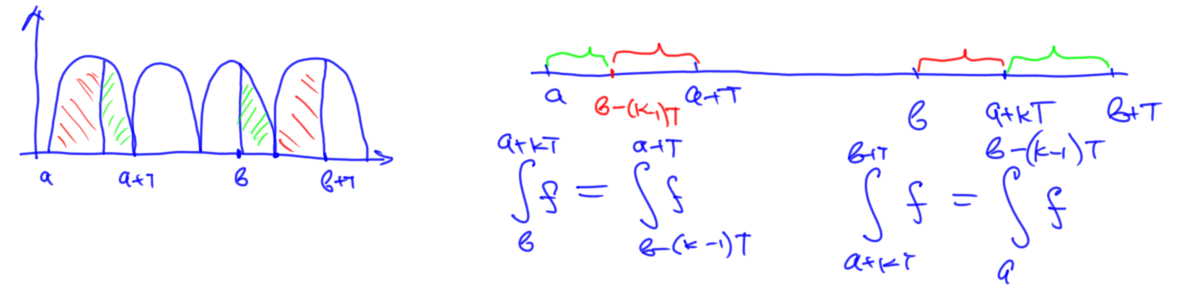
\includegraphics[scale=0.6]{abels_consequence}
    \end{figure}
    
    %$\int\limits_a^{a+kT}f = \int_{b-(k-1)T}^{a+T}f$.  $\int\limits_{a+kT}^{b+T} f = \int\limits_{a+T}^{b-(k-1)T} f$
\end{proof}
\begin{consequence}
   $f, g\in C[a;+\infty)$,  $f$ --- периодическая с периодом  $T$,  $g$ монотонная и $g \xrightarrow{x \to +\infty} 0$  $\int\limits_a^{+\infty} g(x) \mathrm{d}x$ расходится. 

   Тогда $\int\limits_a^{+\infty} fg$ сходится  $\iff \int\limits_a^{a+T} f = 0$.
\end{consequence}
\begin{proof}
    $\Leftarrow$.  $F(x) = \int\limits_a^x f$ --- периодична с периодом  $T$:  $F(x+T) = \int\limits_a^{x+T} f = \int\limits_a^x f + \int\limits_x^{x+T}f = F(x)$.  $F$ --- непрерывна и периодична  $\implies$ ограничена  $\implies$  $\int\limits_a^{+\infty} fg$ сходится по признаку Дирихле.

    $\Rightarrow$. Пусть  $\int\limits_a^{a+T} f \eqqcolon K \neq 0$.  $\widetilde{f}(x) \eqqcolon f(x) - \frac{K}{T}$ --- периодична с периодом $T$. Тогда  $\int\limits_a^{a+T} \widetilde{f} = \int\limits_a^{a+T}(f-\frac{K}{T}) = K - T \cdot \frac{K}{T} = 0 \implies \int\limits_a^{+\infty} \widetilde{f}g$ сходится.

    Тогда $\int\limits_a^{+\infty} fg = \int\limits_a^{+\infty}(\widetilde{f} + \frac{K}{T})g = \int\limits_a^{+\infty} \widetilde{f}g + \frac{K}{T}\int\limits_a^{+\infty} g \implies \int\limits_a^{+\infty} fg$ расходится как сумма сходящегося и расходящегося. 
\end{proof}
\begin{example}
    Рассмотрим $\int\limits_a^{+\infty} \frac{\sin x}{x^p} \mathrm{d}x$.
    \begin{enumerate}
    \item $p > 1$ интеграл сходится абсолютно:  $|\sin x| \le 1 \implies \left| \frac{\sin x}{x^p} \right| \le \frac{1}{x^p}$, а значит $\int\limits_a^{+\infty} \frac{\mathrm{d}x}{x^p}$ сходящийся.
    \item $0 < p \le 1$ интеграл сходящийся, но не абсолютно. $\int\limits_a^{+\infty} \frac{\mathrm{d}x}{x^p}$ --- расходится, $\frac{1}{x^p} \searrow 0$. $g(x) \coloneqq \frac{1}{x^p}, f(x) = \sin x$. $\int\limits_0^{2\pi} \sin x \mathrm{d}x = 0 \implies \int_1^{+\infty} \frac{\sin x}{x^p} \mathrm{d}x$ сходящийся.

        Если взять $f(x) = |\sin x|$, то интеграл по периоду равен  $4$. Значит исходный интеграл расходится.
    \item $p \le 0$ интеграл расходится. 

        $a_n \coloneqq \frac{\pi}{6} + 2\pi n, b_n \coloneqq \frac{5\pi}{6} + 2\pi n$. Тогда $\int\limits_{a_n}^{b_n} \frac{\sin x}{x^p} \mathrm{d}x \ge \frac{1}{2} \int\limits_{a_n}^{b_n} \frac{\mathrm{d}x}{x^p} \ge \frac{1}{2} \int\limits_{a_n}^{b_n} = \frac{b_n - a_n}{2} = \frac{\pi}{3}$. \\
        (предъявили сколь угодно далеко такие отрезки, что интеграл по ним превосходит $\frac{\pi}{3}$ - это отрицание критерия Коши)
    \end{enumerate}
\end{example}
%END TICKET 24
